% Intended LaTeX compiler: pdflatex
\documentclass[presentation]{beamer}
\usepackage[utf8]{inputenc}
\usepackage{lmodern}
\usepackage[T1]{fontenc}
\usepackage{fixltx2e}
\usepackage{graphicx}
\usepackage{longtable}
\usepackage{float}
\usepackage{wrapfig}
\usepackage{rotating}
\usepackage[normalem]{ulem}
\usepackage{amsmath}
\usepackage{textcomp}
\usepackage{marvosym}
\usepackage{wasysym}
\usepackage{amssymb}
\usepackage{amsmath}
\usepackage[theorems, skins]{tcolorbox}
\usepackage[version=3]{mhchem}
\usepackage[numbers,super,sort&compress]{natbib}
\usepackage{natmove}
\usepackage{url}
\usepackage{minted}
\usepackage{underscore}
\usepackage[linktocpage,pdfstartview=FitH,colorlinks,
linkcolor=blue,anchorcolor=blue,
citecolor=blue,filecolor=blue,menucolor=blue,urlcolor=blue]{hyperref}
\usepackage{attachfile}
\usetheme{default}
\author{Jan Boone, Minke Remmerswaal, and Bram Wouterse}
\date{\today}
\title{Health Care Expenditures}
\begin{document}

\begin{frame}{Outline}
\setcounter{tocdepth}{1}
\tableofcontents
\end{frame}


\begin{frame}[label={sec:org8a489c8}]{Introduction}
\begin{block}{Motivation}
\begin{itemize}
\item worries about level/growth healthcare expenditures
\item demand side cost sharing contains expend.
\item currently 385 euros mandatory deductible in NL
\item trade off demand side cost-sharing:
\begin{itemize}
\item lower expenditures
\item higher out-of-pocket for "sick" people
\end{itemize}
\item find \emph{form} of demand side cost sharing to alleviate this trade off?
\end{itemize}
\end{block}

\begin{block}{forms of cost sharing}
\begin{itemize}
\item popular with Dutch policy makers:
\begin{itemize}
\item deductible
\item co-payment (say 25\%)
\item shifted deductible ("donut")
\end{itemize}
\item CPB is supposed to "predict" healthcare expenditures under different schemes
\end{itemize}
\end{block}

\begin{block}{cost sharing}
\begin{figure}[htbp]
\centering
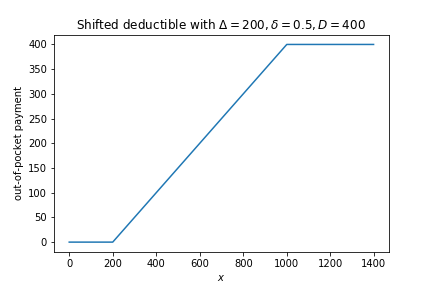
\includegraphics[width=250px]{./shiftedD.png}
\caption{\label{fig:shiftedD}
Out-of-pocket payments with a shifted deductible.}
\end{figure}
\end{block}


\begin{block}{Research question}
\begin{itemize}
\item what are the effects of different cost-sharing \emph{schemes} on healthcare spending?
\item difficulty: after the reform, the Netherlands has only featured deductibles
\item so we can estimate \(y_{it} = ... + \alpha D_t + \varepsilon_{it}\)
\item but cannot determine effect of a 25\% co-payment
\end{itemize}
\end{block}

\begin{block}{Method}
\begin{itemize}
\item use Bayesian estimation techniques to determine distributions of healtcare costs (per age-gender category)
\item determine (expected) out-of-pocket payment (OOP) for each category
\item determine effect of OOP on healthcare expenditures
\item then for each \emph{scheme} we determine OOP and then expenditures
\end{itemize}
\end{block}

\begin{block}{Why Bayesian?}
\begin{itemize}
\item distributions of healthcare spending are important for cost-sharing schemes
\item "standard" econometrics is based on sampling variation
\begin{itemize}
\item but we have data on the whole population
\end{itemize}
\item we want policy recommendations that include uncertainty
\item Bayesian approach can easily work with distributions
\item it is fun!
\end{itemize}
\end{block}

\begin{block}{Policy recommendation}
\begin{itemize}
\item distribution of expenditures for given parameters
\item distribution of parameter values
\end{itemize}
\begin{figure}[htbp]
\centering
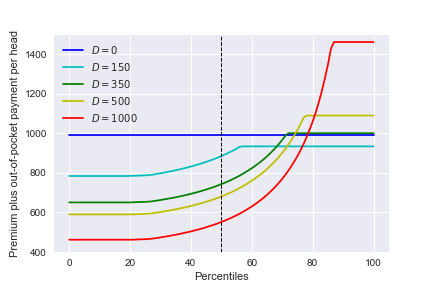
\includegraphics[width=900px]{./deciles_deductible_male_female_Healthy.png}
\caption{Trade offs increasing deductible}
\end{figure}
\end{block}

\begin{block}{Distributions}
\begin{figure}[htbp]
\centering
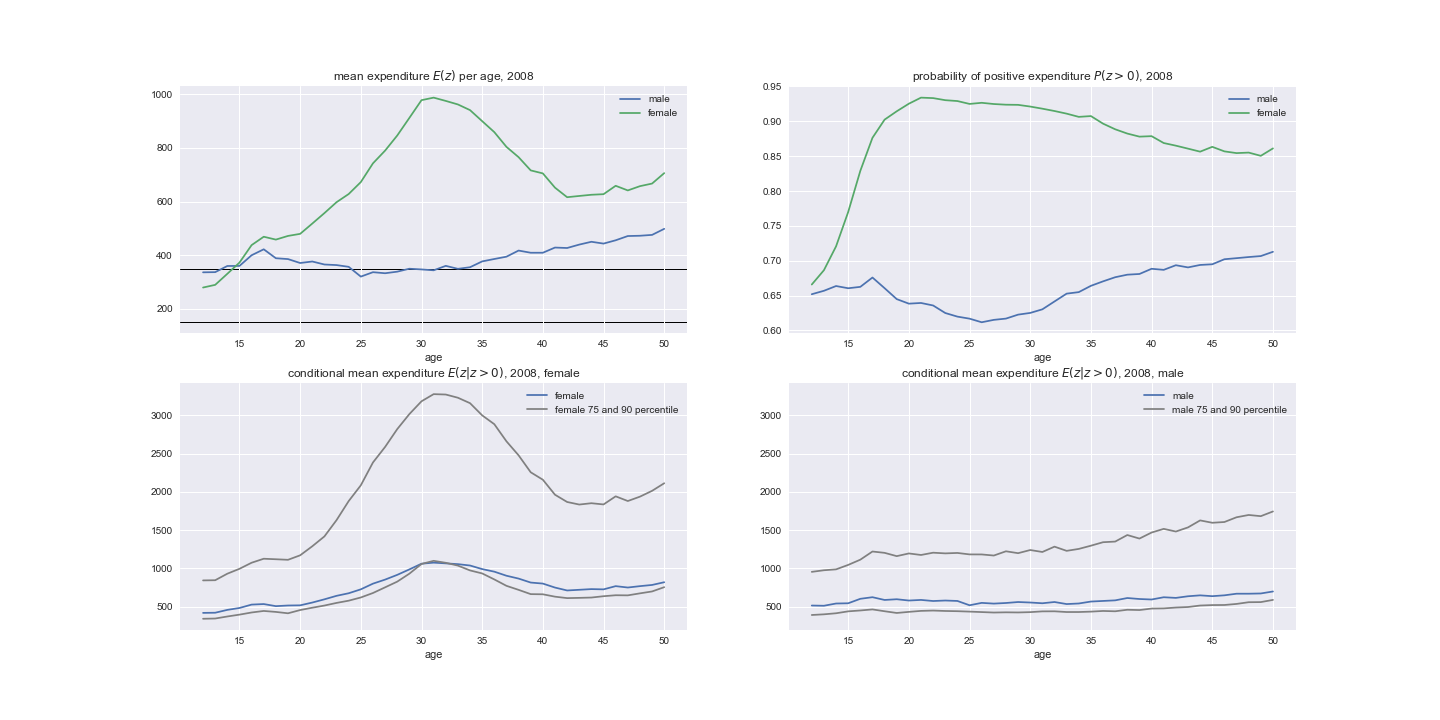
\includegraphics[width=500px]{./ExpenditureOverAge.png}
\caption{Expenditure distributions}
\end{figure}
\end{block}
\end{frame}

\begin{frame}[label={sec:orgbfe8ad2}]{Literature}
\begin{block}{Modeling healthcare expenditures}
\begin{itemize}
\item Einav et al. (2013)
\item Hayen et al. (2019)
\item Remmerswaal et al. (2019)
\end{itemize}
\end{block}
\end{frame}

\begin{frame}[label={sec:org8b91621}]{Model}
\begin{block}{Simple model}
\begin{itemize}
\item one treatment per period: cost and value
\end{itemize}
\begin{center}
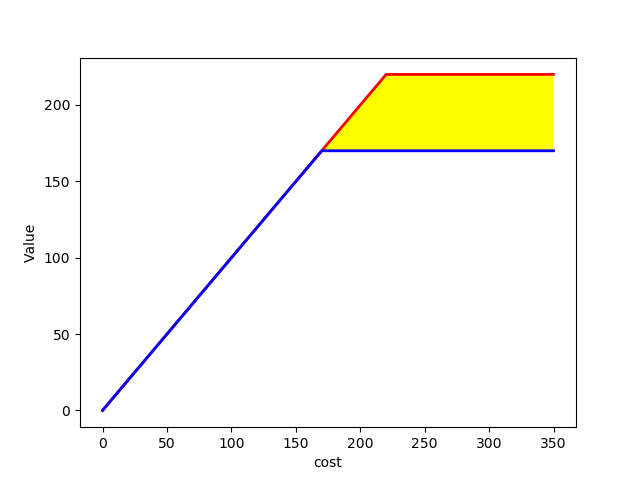
\includegraphics[width=250px]{./deduct.png}
\end{center}
\end{block}

\begin{block}{Total healthcare expenditure in a year}
\begin{itemize}
\item \(H(z)\): distribution of healthcare expenditure in a year
\begin{itemize}
\item where \(z=x+y\)
\item \(x\): exogenous, not affected by cost-sharing, high-value care
\begin{itemize}
\item if you break your leg, you get "plastered up"
\end{itemize}
\item \(y\): endogenous, affected by cost-sharing
\begin{itemize}
\item if you have a running injury, perhaps you skip the physiotherapy
\end{itemize}
\end{itemize}
\end{itemize}
\end{block}

\begin{block}{Idea of the model}
\begin{itemize}
\item "at the start of the year", person \(i\) is offered one \(y\) treatment with value \(v_y\) and expected out-of-pocket \(OOP\)
\item \(i\) accepts if \(v_y\) exceeds expected \(OOP\)

\item \(OOP\) depends on:
\begin{itemize}
\item \(f(x)\) ex-ante distribution of exogenous healthcare expenditure
\item \(g(y)\) cost distribution of offered treatment \(y\)
\item cost-sharing scheme
\end{itemize}
\item for a deductible \(D\), \(OOP\) equals \(\int_0^{+\infty} \int_0^{+\infty} (\min\{x+y,D\}-\min\{x,D\})f(x)g(y)dxdy\)
\end{itemize}
\end{block}
\end{frame}


\begin{frame}[label={sec:orga870408}]{Data}
\begin{block}{Dutch healthcare expenditure}
\begin{itemize}
\item expenditures per individual for 2008-2013
\item we use indiv.'s age and gender
\item later add income, indicators for health status
\item expenditures are for basic insurance under the deductible (e.g. not GP)
\item basic insurance is mandatory in the Netherlands
\item coverage is set by the government
\item we ignore people with voluntary deductible (for the moment)
\item deductible "kicks in" at 18
\end{itemize}
\end{block}
\end{frame}

\begin{frame}[label={sec:org025e19e},fragile]{Estimation}
 \begin{block}{Parametric specification}
\begin{itemize}
\item "everybody knows" that healthcare expenditures are log-normally distributed:
\begin{itemize}
\item log transformation of positive healthcare costs are normally distributed
\item we model the propability of zero healthcare costs
\item benefits of log-normal distribution:
\begin{itemize}
\item analytical expression for \(OOP\) with deductible (estimation)
\item analytical expression for distribution of \(x+y\)
\end{itemize}
\end{itemize}
\end{itemize}
\end{block}

\begin{block}{Two distributions}
\begin{figure}[htbp]
\centering
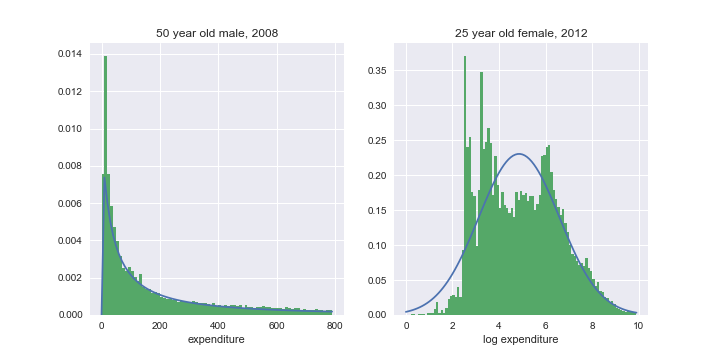
\includegraphics[width=.9\linewidth]{./DistributionExpenditure.png}
\caption{\label{fig:TwoDistributions}
Illustrative distributions for \emph{positive} healthcare costs (left in levels, right in logs)}
\end{figure}
\end{block}

\begin{block}{Four components}
\begin{itemize}
\item define categories age by gender
\begin{itemize}
\item each category \emph{distribution} (log) healthcare costs \(z\)
\end{itemize}
\item distribution is mixture:
\begin{itemize}
\item \(x \sim N(\mu_x,\Sigma_x)\), given gender a Gaussian Process with age; year fixed effects
\item same for \(y\)
\item \(\psi\) is probability treatment is offered (\(x > 0\)), GP with age
\item \(\phi\) is same for \(y > 0\)
\end{itemize}
\end{itemize}
\end{block}

\begin{block}{OOP}
\begin{itemize}
\item people in each category know their \(\psi,\phi\) and their distributions of \(x,y\)
\item calculate \(OOP\) per age, gender, year with \(x,y,\psi,D\)
\item compute probability \(F\) that \(y\) is rejected (\(v_y < OOP\))
\begin{itemize}
\item \(F(OOP) = 1-\zeta e^{-\nu*OOP}\)
\end{itemize}
\end{itemize}
\end{block}

\begin{block}{Probabilities}
\begin{itemize}
\item calculate probability for each mixture component
\end{itemize}
\begin{center}
\begin{tabular}{ll}
component & probability\\
\hline
\(x=y=0\) & \((1-\psi)(1-\phi + \phi F)\)\\
\(x>0=y\) & \(\psi*(1-\phi + \phi F)\)\\
\(y>0=x\) & \((1-\psi)\phi(1-F)\)\\
\(x,y>0\) & \(\psi \phi (1-F)\)\\
\end{tabular}
\end{center}
\end{block}

\begin{block}{Training vs validation data}
\begin{itemize}
\item we split the data in training, validation and test
\item we estimate on training
\item check fit with validation
\item look at test set once we are finished
\end{itemize}
\end{block}

\begin{block}{Technique}
\begin{itemize}
\item specify priors for parameters:
\begin{itemize}
\item 5,000,000 observations per year
\item on average 65,000 observations per category per year
\end{itemize}
\item estimation with variational inference (ADVI, Auto-diff Variational Inference) and minibatches
\begin{itemize}
\item Markov Chain Monte Carlo methods (Metropolis, NUTS etc.) do not scale well
\end{itemize}
\item python and pymc3 fun to work with
\begin{itemize}
\item parameter \(\phi\) has age fixed effects: \texttt{ϕ[age]}
\end{itemize}
\end{itemize}
\end{block}

\begin{block}{Posterior}
\begin{itemize}
\item for each age-gender category, we draw 10,000 samples of the model parameters
\item for each sample we draw one \(x,y\) and \(z\)
\item that is, we draw outcomes (not averages or expectations)
\item use the whole posterior distribution, not only the mode
\end{itemize}
\end{block}

\begin{block}{More formally}
\begin{itemize}
\item parameters \(\theta\)
\item data \(y\)
\item posterior:
\end{itemize}
\begin{equation}
Pr(\theta|y) = \frac{Pr(y|\theta)Pr(\theta)}{Pr(y)} = \frac{Pr(y|\theta)Pr(\theta)}{\int Pr(y|\theta)Pr(\theta)d\theta }
\end{equation}
\begin{itemize}
\item we simulate this posterior ("samples")
\item for each sample, we generate an outcome (i.e. expenditure level)
\end{itemize}
\end{block}
\end{frame}

\begin{frame}[label={sec:org1abe136}]{Fit}
\begin{block}{How to measure fit}
\begin{itemize}
\item not obvious how to measure the fit of the model
\item we can compare: 
\begin{itemize}
\item average expenditure per age-gender category (fit vs validation data)
\item expenditure distributions per age-gender categories
\item predicted vs realized (validation) zero-expenditures per category
\end{itemize}
\end{itemize}
\end{block}

\begin{block}{Fit on average (log) costs by age and year: Men}

\end{block}

\begin{block}{Fit on average (log) costs by age and year: Women}

\end{block}

\begin{block}{Expenditure distributions}
\begin{figure}[htbp]
\centering
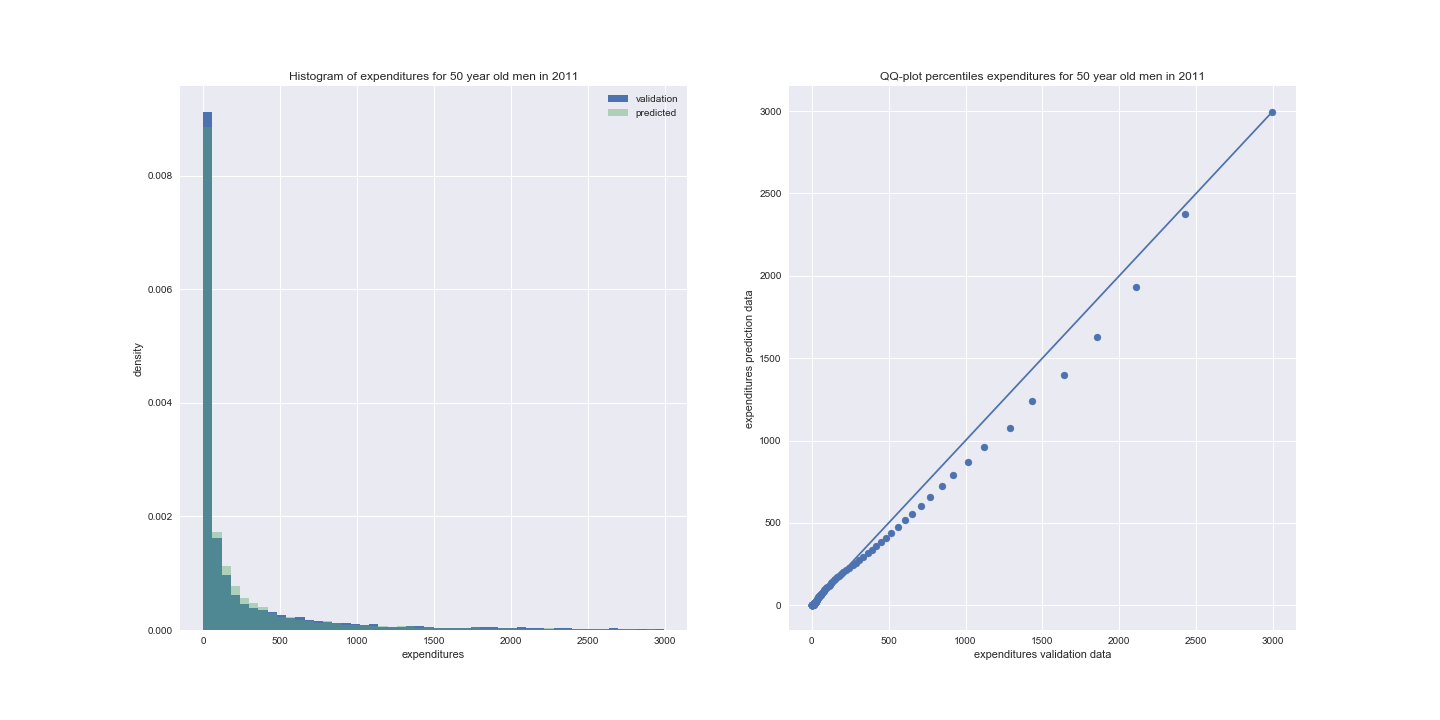
\includegraphics[width=500px]{./PredictedvsValidationDistributions_healthy_Male.png}
\caption{\label{fig:predictedvsValidationDistributions}
Predicted vs validation}
\end{figure}
\end{block}

\begin{block}{Probability positive expenditures}
\begin{figure}[htbp]
\centering
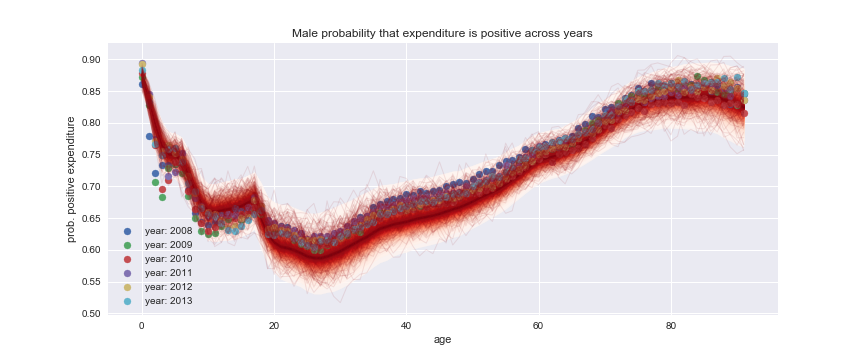
\includegraphics[width=500px]{./PredictedPositiveExpenditureAcrossAge_healthy_Male.png}
\caption{\label{fig:predictedposexpend}
Predicted and realized probabilities of positive expenditures for men across age and years.}
\end{figure}
\end{block}
\end{frame}


\begin{frame}[label={sec:org529e4a1}]{Simulations}
\begin{block}{Samples}
\begin{itemize}
\item we use \(F(OOP) = 1-\zeta e^{-\nu OOP}\)
\item is the estimate for \(\nu\) "significant"?
\end{itemize}

\begin{figure}[htbp]
\centering
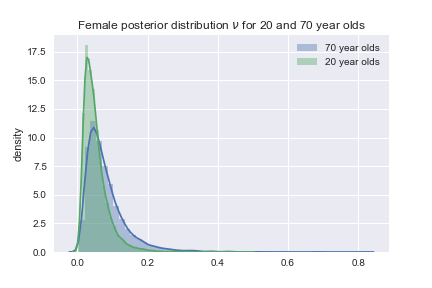
\includegraphics[width=250px]{./Posterior_nu_y_healthy_Female.png}
\caption{\label{fig:nu_women}
Posterior distribution of \(\nu\) for women}
\end{figure}
\begin{itemize}
\item we have these distributions for each parameter
\end{itemize}
\end{block}





\begin{block}{Deductible: average effect}
\begin{figure}[htbp]
\centering
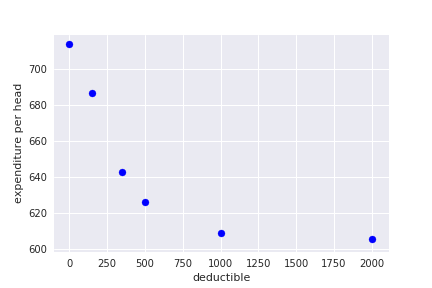
\includegraphics[width=250px]{./Population_weighted_average_exp_simulation_deductibles_healthy_Male.png}
\caption{\label{fig:exp_deduc}
Average healthcare expenditures per capita for different deductibles.}
\end{figure}
\end{block}


\begin{block}{Deductible: uncertainty average effect}
\begin{figure}[htbp]
\centering
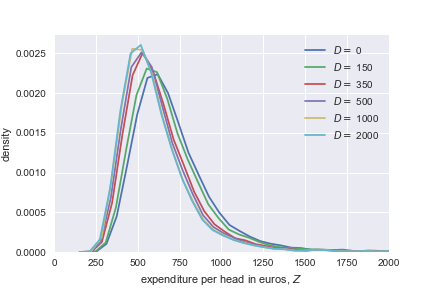
\includegraphics[width=250px]{./Density_plots_simulation_deductibles_healthy_Male.png}
\caption{\label{fig:exp_deduc}
Distribution average healthcare expenditures per capita for different deductibles.}
\end{figure}
\end{block}


\begin{block}{Deductible: distribution effects}
\begin{figure}[htbp]
\centering
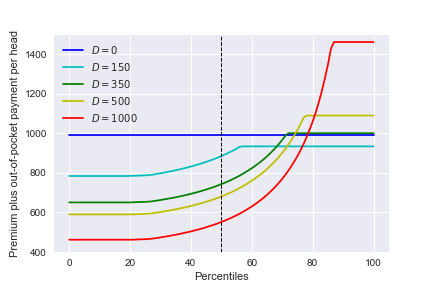
\includegraphics[width=900px]{./deciles_deductible_male_female_Healthy.png}
\caption{Trade offs increasing deductible}
\end{figure}
\end{block}
\end{frame}


\begin{frame}[label={sec:org22618ff}]{Conclusion}
\begin{block}{Summary}
\begin{itemize}
\item in order to determine healthcare expenditures under different cost sharing schemes:
\begin{itemize}
\item we estimated the distributions of healthcare expenditures
\item split expenditures up in exogenous and endogenous expenditures
\end{itemize}
\end{itemize}
\end{block}

\begin{block}{Summary (cont)}
\begin{itemize}
\item determined expected OOP for endogenous expenditures under different schemes
\item estimate the value distribution of these endog. expenditures
\item the higher OOP, the more likely an (endogenous) treatment is rejected
\item allows us to simulate effects of different \emph{schemes}
\end{itemize}
\end{block}

\begin{block}{Policy recommendations}
\begin{itemize}
\item Bayesian analysis allows us to:
\begin{itemize}
\item work with posterior \emph{distribution} of parameters
\begin{itemize}
\item instead of just the mode (or mean)
\end{itemize}
\item present uncertainty about each "object"
\begin{itemize}
\item parameter estimate
\item average effect
\end{itemize}
\item distribution effects include:
\begin{itemize}
\item uncertainty of expenditures for given parameter values
\item uncertainty about parameter values
\end{itemize}
\end{itemize}
\end{itemize}
\end{block}

\begin{block}{Robust recommendation}
\begin{itemize}
\item having a small but strictly positive deductible makes \emph{everyone} better off compared to zero deductible
\item because the deductible reduces expenditures, it reduces the insurance premium
\item to such an extent that even people with the highest expenditures are better off than with no deductible
\item higher deductibles reduce expenditures further, but "sick" people than have higher out-of-pocket payments
\end{itemize}
\end{block}
\end{frame}
\end{document}